\documentclass[t]{beamer}
\usepackage{CJKutf8}
\usepackage{amsfonts}
    \usepackage{amsmath}
    \usepackage{amssymb}
    \usepackage{amsthm}
    \usepackage{enumerate}
    \usepackage{graphicx}
    \usepackage{layout}
    \usepackage{mathrsfs}
    \usepackage{fancyhdr}
    \usepackage{subfigure}
    \usepackage{tcolorbox}
    \usepackage{tikz-cd}
    \usepackage{color}
    \usepackage{pifont}
    \usepackage{verbatim}
    \usepackage{mathtools}
    \usepackage{float}
    \usepackage{bm}
    \usetheme{AnnArbor}
% \usetheme{Antibes}
\usecolortheme{beaver}
% 表格
\usepackage{booktabs}
\usepackage{multirow}

% \setbeamertemplate{navigation symbols}{}

\usepackage{textpos}

\newcommand{\dif}{\mathrm{d}}
\newtheorem{thm}{{定理}}




\begin{document}
\begin{CJK*}{UTF8}{gkai}
% 一般第一页显示PPT标题以及作者信息

% \BackgroundPic{./Screenshot from 2022-04-20 16-31-08.png}

% 增加学校 前面
\addtobeamertemplate{title page}{}{
	\begin{tikzpicture}[remember picture,overlay]
		% \node[yshift=85pt,xshift=50pt]{\includegraphics[height=2cm]{Screenshot from 2022-04-20 16-51-21.png}};
\end{tikzpicture}
}


	\title{NLP模型汇报}
	\subtitle {} %不需要
	\author{
		陈钶杰\, \\
		专业:计算数学\,
	} % 显示作者
	% \institute {学院:数学科学学院} % 设置学院机构	
	\date{\today}  % 显示日期
\titlepage

% 设置目录
\begin{frame}{目录}
\frametitle{目录}	
\tableofcontents  % 显示目录
\end{frame} 

\newcommand{\eee}[1]{\begin{enumerate}#1\end{enumerate}}

\section{transformer模型}


\begin{frame}
	\frametitle{tranformer模型}
    \begin{itemize}
		\item
		\textcolor{red}{介绍:}
		\begin{itemize}
		\item Transformer是一种基于注意力机制的神经网络架构,最初用于处理序列到序列(Sequence-to-Sequence)的任务,如机器翻译。
		\item Transformer在处理长序列时具有更好的并行性和捕捉长距离依赖关系的能力。
		\end{itemize}
	\end{itemize}
\end{frame}

\begin{frame}
	\frametitle{transformer模型}
    \begin{itemize}
		\item 模型的基本框架\\
		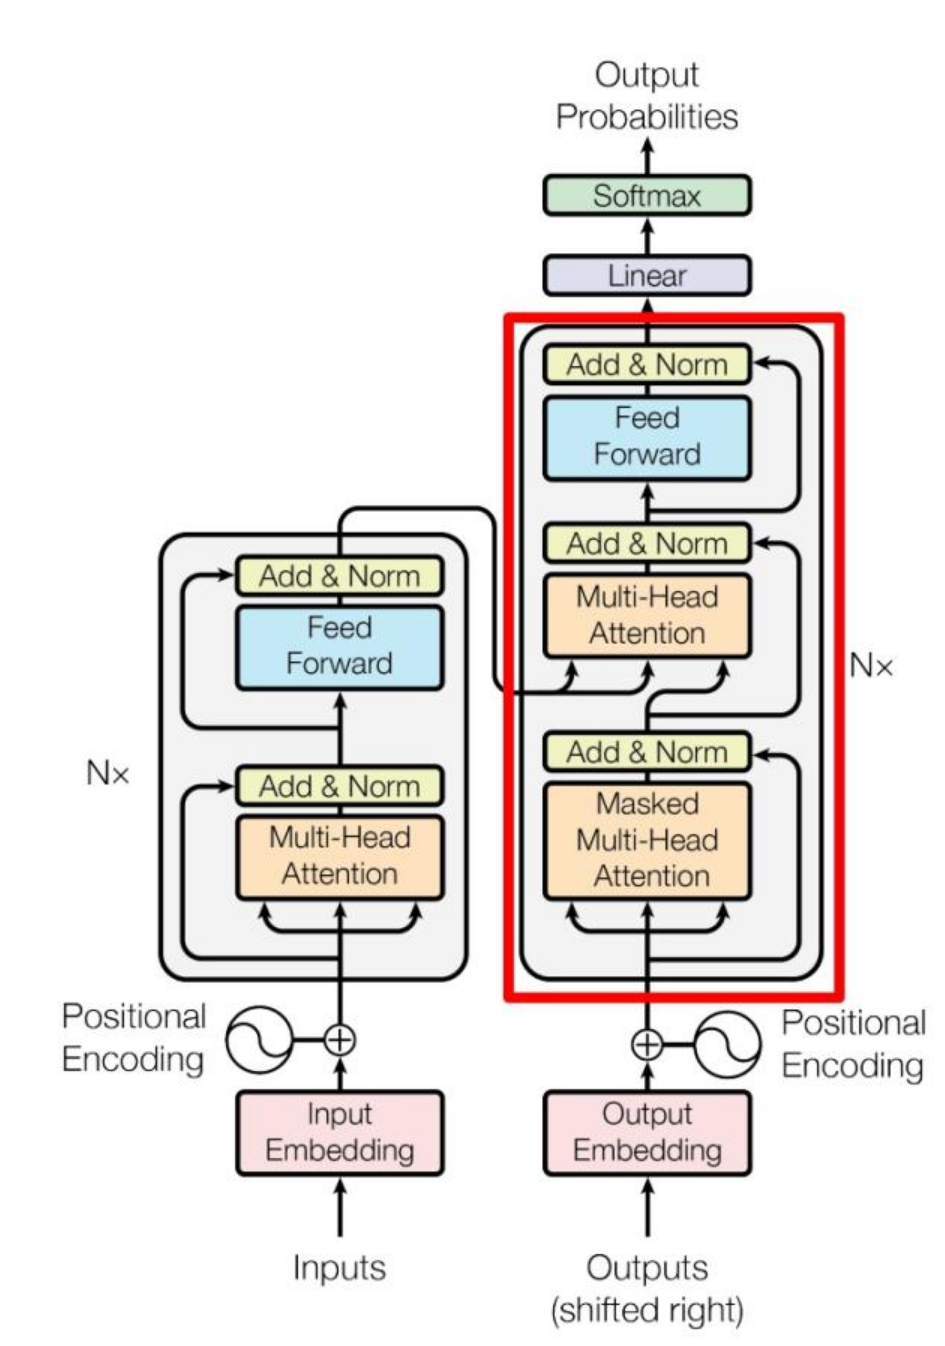
\includegraphics[scale=0.1]{png/tranformer.png}
		\end{itemize}
\end{frame}


\begin{frame}	
	\begin{itemize}
		\item
		进行中英文翻译举例(使用pytorch):\\
		\textcolor{red}{预训练过程}:
		\begin{itemize}
			\item input:中文词汇表,英文词汇表,中英文句子对应表\\
				output:模型的所有参数
		\end{itemize}
		\textcolor{red}{具体流程}:
		\begin{itemize}
			\item Encoder
			\begin{enumerate}
				\item 使用torch的内置嵌入函数,将输入的中文句子中的每个单词转换为一个向量,并结合单词在句子中的位置向量,得到最终的信息表示。
				% 将输入的中文句子使用torch的内置嵌入函数将每个单词变成一个向量,再添加单词在句中的位置向量得到最终的信息.
				\item 使用多头注意力机制(MultiHeadAttention),核心是将单词的表示向量拆分成多个子空间。通过使用矩阵运算,该注意力机制可以有效地捕捉句子中不同单词之间的关系。这种关系可以帮助模型更好地理解上下文信息,从而提高模型在处理自然语言任务中的性能。
				% 使用多头注意力机制(MultiHeadAttention),核心是将单词的维度拆分多分.这个注意力机制的可以通过使用矩阵得到句子中的上下词之间的关系.
				\item 将上一步得到的结果输入前馈神经网络(Feed-Forward Neural Network),这一步在最终效果的呈现中起到关键作用。前馈神经网络通过多层感知机(Multi-Layer Perceptron, MLP)结构,对输入进行非线性变换和映射。这种变换能够增强特征的表达能力和复杂性,从而提高模型的性能和表现。
				% 将上一步结果输入到前馈神经网络.这一步对于最终效果的呈现起到关键作用.
			\end{enumerate}
		\end{itemize}
	\end{itemize}
\end{frame}

\begin{frame}
	\textcolor{red}{具体流程}:	
	\begin{itemize}
		\item Deconder
		\begin{enumerate}
			\item 使用torch的内置嵌入函数,将输入的英文句子中的每个单词转换为一个向量,并结合单词在句子中的位置向量,得到最终的信息表示。
			\item 使用多头注意力机制(MultiHeadAttention),但是这边与编码器中的多头注意力机制相比,有些不同,即解码器有两种不同的多头注意力机制.
			\item 第一是需要MASK,希望通过MASK使得一句话只受前面信息的影响,而不会受到后面内容的影响.
			\item 第二种不同之处在于第二层的多头注意机制通过使用编码器中的值(V)、键(K)以及解码器中第一层得到的查询(Q),来建立中英文之间的关系。这一步可以帮助模型更好地捕捉并联系中英文之间的语义和上下文关系,从而提高模型在翻译和跨语言任务中的性能。
			% 第二个不同在于第二层的多头注意机制是通过使用编码器里面的Q,K,以及解码器得到的V.这一步可以将中英文之间的关系联系起来.
			\item 将上一步得到的结果输入前馈神经网络
		\end{enumerate}
		\item 预测输出单词
		\begin{enumerate}
			\item 使用softmax得到句中每个单词对应词汇表中所有单词的概率.
		\end{enumerate}
	\end{itemize}	
\end{frame}	

\begin{frame}
	\textcolor{red}{使用的损失函数:交叉熵}	\\
	\begin{itemize}
		\item 对于多分类问题,交叉熵损失函数的定义如下:
		$$
			L_{CE} = - \sum_{i=1}^{N} y_i \log(p_i)
		$$
		其中,$y_i$是真实标签的one-hot编码,$p_i$是模型对类别i的预测概率。\\
	\end{itemize}
	
\textcolor{red}{迭代计算}	\\
\begin{itemize}
	% \item  通过从具有最大概率的单词中组成句子,并计算其与原始输入英文句子之间的交叉熵,进行误差反向传播和参数更新。通过多次迭代,目标是使结果尽可能准确。
	\item 在这个过程中,模型会根据输入句子生成一个输出序列,然后将其与目标输出进行比较。通过计算交叉熵损失函数,可以衡量模型的输出与目标之间的差异。接下来,误差会通过反向传播算法传递回模型,更新模型的参数,以使输出逐渐接近目标。
	\item 	通过多次迭代训练,模型会不断调整参数,提高其性能和准确度。最终目标是使模型生成的句子与目标输出尽可能一致,并且交叉熵损失尽可能小。这样,模型就能够学习到语言的结构和语义,并生成更准确和有意义的句子。
\end{itemize}

\end{frame}	

% section一定要写在frame框架的上面
\section{BERT模型}

\begin{frame}
	\frametitle{BERT模型}
    \begin{itemize}
		\item
		\textcolor{red}{介绍:}
		\begin{itemize}
		\item BERT是一个能处理各种自然语言任务(NLP)的通用架构,该模型主要目标是通过在大规模无标签文本上进行预训练,学习通用的语言表示.
		\item 主要功能:\\
		\begin{enumerate}
			\item 遮蔽语言模型(完型填空):在遮蔽语言模型任务中,BERT会将整个输入句子输入模型,并随机遮蔽一部分单词。模型需要通过上下文中的其他单词来预测被遮蔽的单词。这样的训练方式使得模型能够学习到上下文间的依赖关系,以及对上下文进行推理和填充的能力。
			\item 下个句子预测:BERT会接收两个连续的句子作为输入,并判断它们是否为原始文本中的下一句。这样的任务有助于模型学习到句子间的关联和逻辑推理能力。
		\end{enumerate}
		\item 此模型是基于tranformer的编码器部分.将一个句子的单词随机遮挡15\%,然后经过多层多头注意力机制,以及前馈神经网络后得到被掩盖词的最有可能值.计算交叉熵,误差通过反向传播算法传递回模型,更新模型的参数,以使输出逐渐接近目标。
		\end{itemize}
	\end{itemize}
\end{frame}


\begin{frame}
	\frametitle{BERT模型}
	\textcolor{red}{	基本框架:}\\
	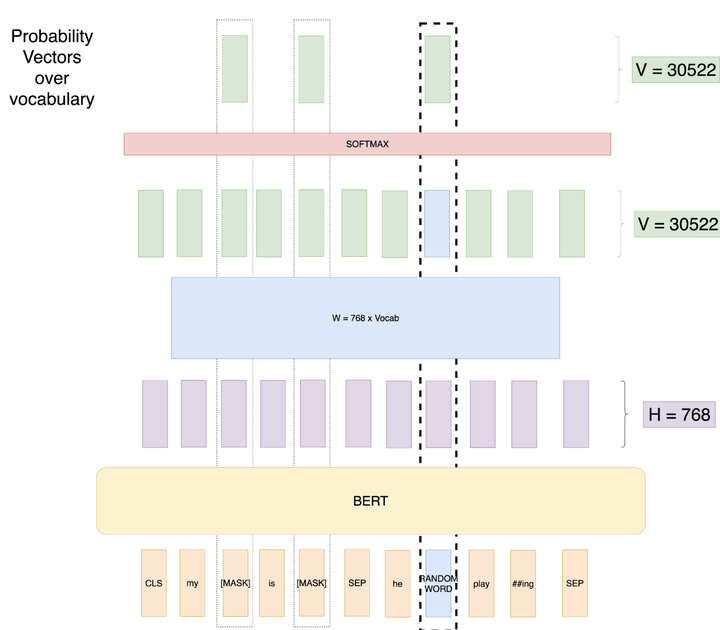
\includegraphics[scale=0.3]{png/bert.png}
\end{frame}


% section一定要写在frame框架的上面
\section{GPT模型}

\begin{frame}
	\frametitle{GPT模型}
    \begin{itemize}
		\item
		\textcolor{red}{介绍:}
		\begin{itemize}
		\item 
		% 预训练模型是指他不使用任务特定样本进行训练的模型,通过在大规模未标记的数据中进行自我训练.而传统的非预处理模型都是通过在人工标记数据后进行训练的.在预训练完成后,预训练模型可以通过微调或迁移学习的方式应用于特定任务,并利用特定任务的要求,并提供更好的性能
		GPT与BERT一样也是一种预训练模型,与BERT不同的是,GPT是一个单向的语言模型,只能根据前面的文本生成下一个词,且GPT使用的是Transformer的Decoder结构。在大量没有标号的数据上训练出一个预训练模型,然后少量有标号的数据上微调训练一个中下游任务的模型。在微调的时候构造与任务相关的输入,就可以很少地改变模型的架构.
		\item gpt模型的主要功能:文本分类,文本预测.
		\item gpt模型的学习的目标函数如下:\\
	$$
    L_1(token_1,...,token_n) = \sum^{N}_{n=K}p(token_n|token_{n-k},...,token_{n-1};\theta)
	$$
	% \item GPT模型的具体是如何运转的?(不是很清楚)		
		\end{itemize}
	\end{itemize}
\end{frame}

\begin{frame}
	\frametitle{GPT模型}
	\textcolor{red}{	基本框架:}\\
	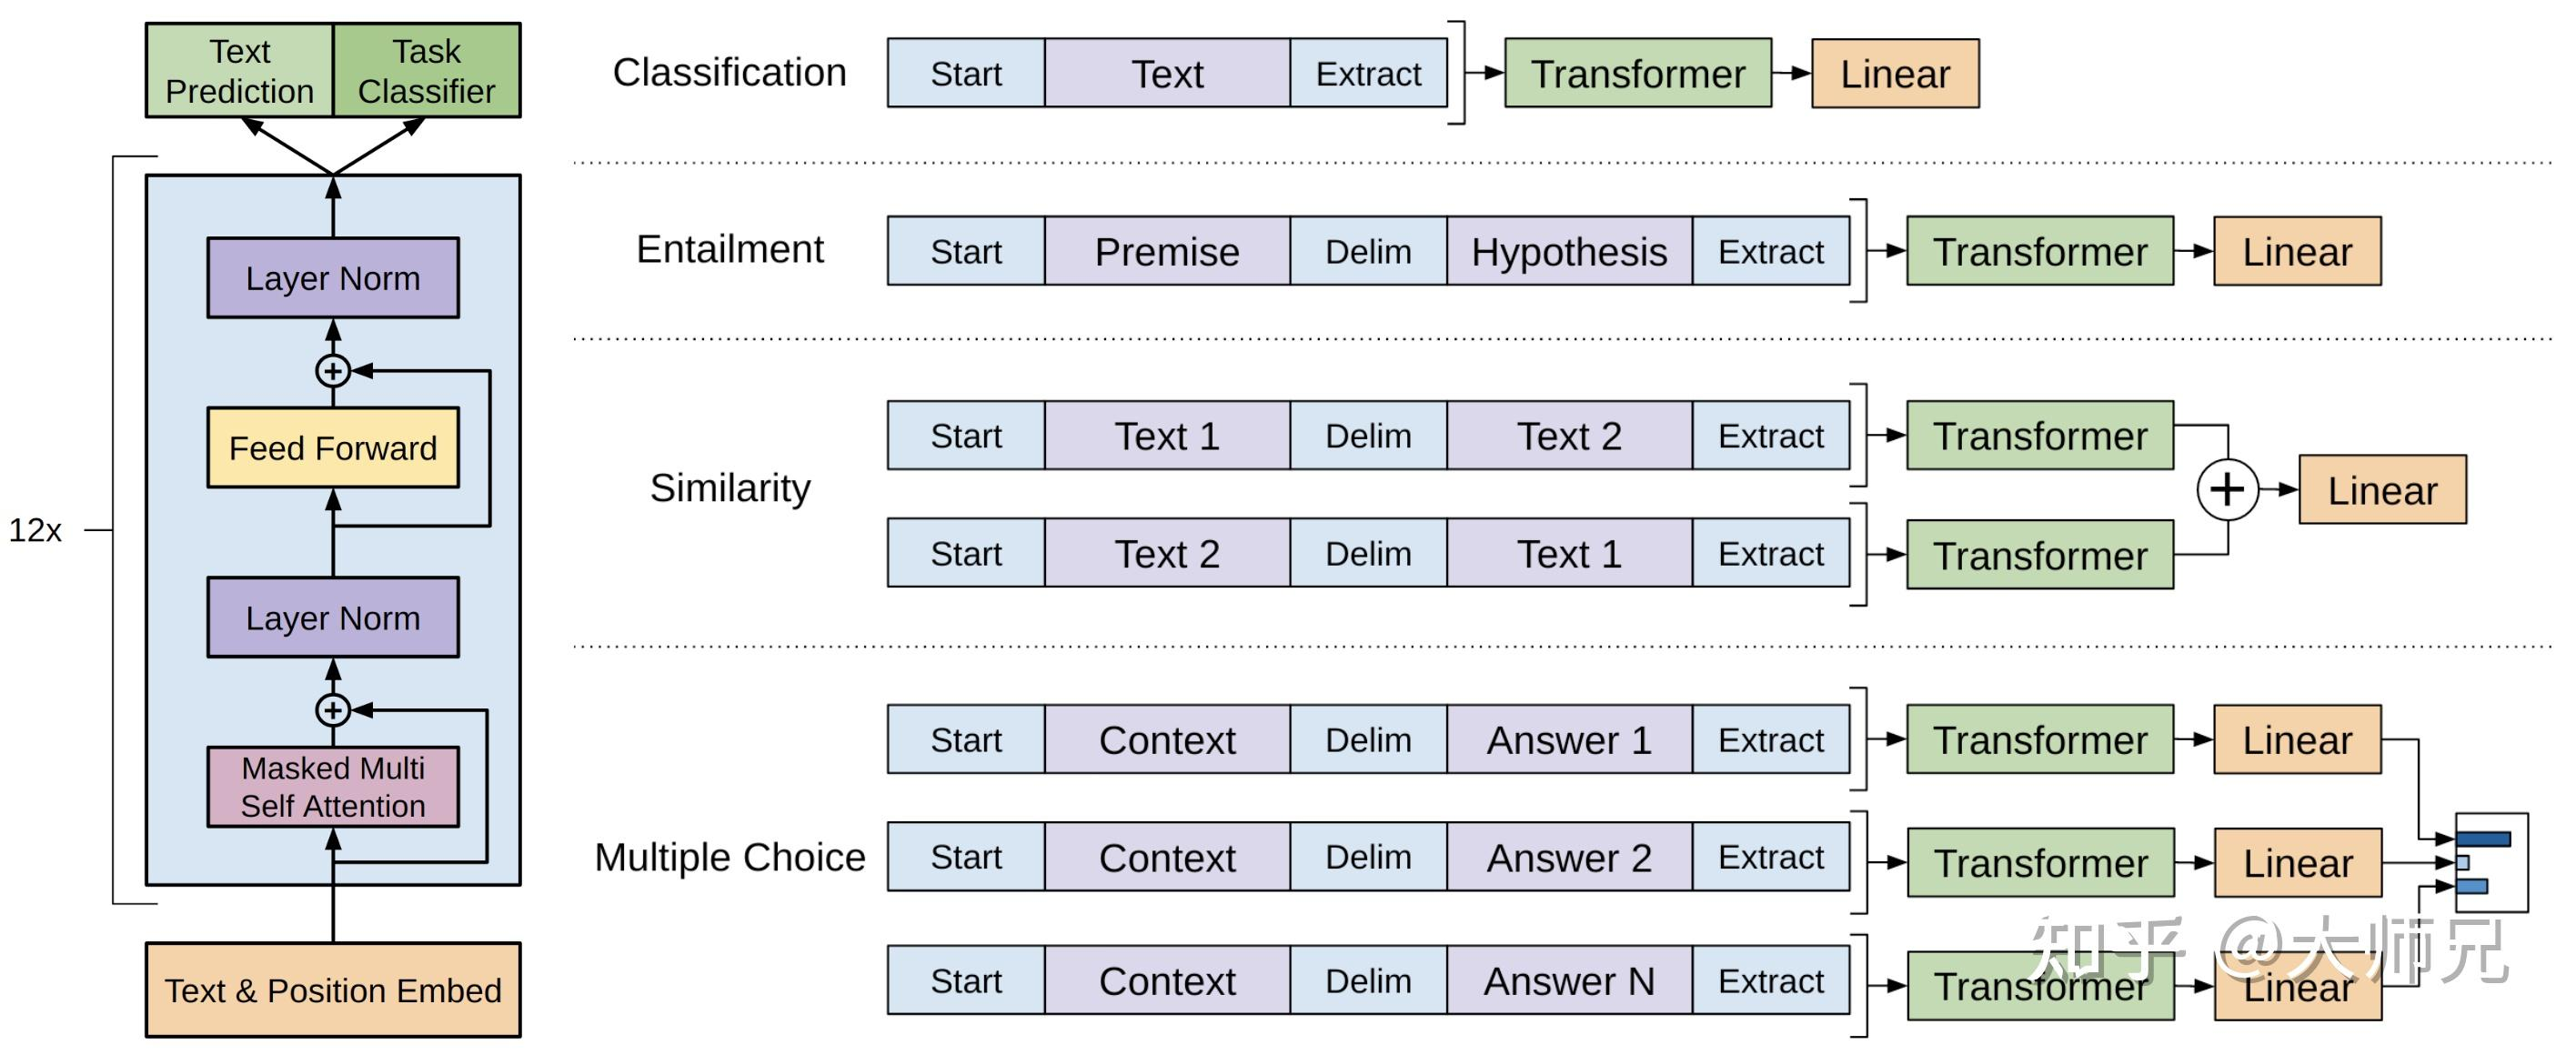
\includegraphics[scale=0.12]{png/gpt.jpg}
\end{frame}


\begin{frame}
	\frametitle{GPT模型}
	\textcolor{red}{GPT的微调模型}\\
	\begin{enumerate}
		\item Fine-tuned(微调)是指在预训练模型的基础上,通过进一步的训练和调整,使模型适应特定任务或数据集的过程。预训练模型(如GPT)通常是在大规模无标注文本上进行训练,学习到了丰富的语言知识和模式。但是,这些预训练模型并不是针对特定任务设计的,因此需要通过Fine-tuning来对模型进行定制化,使其在特定任务上表现更好。
		\item 经过预训练的模型并不能做到情感分类,即给定一段文本,判断其是积极的还是消极的。我们可以使用GPT模型进行Fine-tuning来解决这个任务。
		\item fine-tuning的训练阶段一般是将基础模型与任务特定的分类层相结合,通常,我们在基础模型之后添加一个全连接层(MLP),后使用交叉熵损失函数来计算模型的预测结果与真实标签之间的差异。
	\end{enumerate}
\end{frame}


\begin{frame}
	\frametitle{如何进行更好的微调?}
	\textcolor{red}{Fine-tuned潜在的缺点}\\
	\begin{enumerate}
		\item 数据需求:GPT的Fine-tuning通常需要大量的任务特定训练数据。为了在特定任务上获得良好的性能,需要提供大规模、高质量的标注数据进行Fine-tuning。这会增加数据收集和标注的成本和工作量。
		\item 灵活性:GPT的Fine-tuning在预训练模型的基础上进行微调的。模型结构和预训练权重是固定的,只能通过微调任务特定层来适应特定任务。这可能限制了模型的灵活性和能力,特别是对于某些复杂或特殊的任务。
	\end{enumerate}
	\textcolor{red}{考虑Prompt learning 替代 Fine-tuning}\\
	\begin{enumerate}
		\item 简单易用:相比于Fine-tuning需要大规模标注数据和复杂的模型调整,Prompt learning更加简单和直观,只需要设计和选择合适的提示。
		\item 灵活性和可解释性:Prompt learning模型可以针对特定任务和领域进行定制,提高模型的适应性和泛化能力。提示是人为设计的,可以使得模型的预测结果更加可解释和可理解。
	\end{enumerate}
\end{frame}


\section{Prompt learning 模型}
\begin{frame}
	\frametitle{Prompt learning 模型}
	\textcolor{red}{ 定义任务和目标:}\\
	\begin{itemize}
		\item 提示学习模型的构建过程(以情感分类为例):\\
			\eee{
				\item 定义任务和目标:首先,确定任务的类型和具体目标。例如,文本生成、翻译、问答等。明确希望模型能够对句子进行情感分类
				\item 将提示与输入结合:在生成过程中,将提示与输入文本或上下文结合起来作为模型的输入。这样,模型能够通过引导提示的方式更好地理解任务和上下文,并生成符合预期的输出。例如将一句话添加提示语句后有"I like the films,it was [mask](提示语句)"
				\item 微调模型:使用提示和相应的数据集对预训练模型进行微调,以适应特定任务和提示。微调过程中,可以使用与任务相关的数据对模型进行训练,以提高模型在任务中的性能。
				\item 生成输出:使用微调后的模型,根据给定的输入和提示进行文本生成。模型会根据上下文和任务要求生成输出文本,并且通过提示来引导生成的过程,以满足特定的预期结果。
				}
	% \item 个人理解:解决情感分析问题(即判断一句话是积极,消极还是中立),对于一个语言模型,本来是通过给一堆句子以及对于句子的判定,然后将这些内容作为输入,判断是否是正确,进行交叉熵的损失函数的计算来得到最终的结果.现在提示模型是这样的通过给定一句话,比如"这是一部关于动物的电影",然后加上"他是xxx",即"这是一部关于动物的电影,他是xxx",把xxx遮挡.然后经过BERT模型就可以得到这个位置对应的各个词的概率.再将这些对应词和情感分析的三种情况做一个映射,就可以进行句子的情感分析了.但是像句子最后加入"他是xxx"这样的内容是比较难的. 
%   \item 上面的"他是xxx"称为pattern(template),而如何构建合适的pattern是Prompt-tuning 的研究热点之一.
%   \eee{
%     \item Patterns ensembling:(同一个句子设置多个不同patterns),比如这个科幻电影,"他是xxx"-"我认为他是xxx"-"评论是xxx",然后xxx只能是great 或者 terrible
%     \item Varbalizers Ensembling:(同一个句子并非一个词可以做标签),比如这个科幻电影,"他是xxx"-"我认为他是xxx",xxx只能是 好 或者 不好,好看,最后映射到 great和terrible
%     \item PVPs Ensembling 结合上面两个,每句话用多个词语形容,然后最后输出.
%     \item 现有的挑选合适的Pattern方法
%     \eee{
%       \item 人工构建(Manual Template) :在前文已经描述过,不再详细说明;
%       \item 启发式法(Heuristic-based Template) :通过规则、启发式搜索等方法构建合适的模板;
%       \item 生成(Generation) :根据给定的任务训练数据(通常是小样本场景),生成出合适的模板;
%       \item 词向量微调(Word Embedding) :显式地定义离散字符的模板,但在训练时这些模板字符的词向量参与梯度下降,初始定义的离散字符用于作为向量的初始化;
%       \item 伪标记(Pseudo Token) :不显式地定义离散的模板,而是将模板作为可训练的参数;
%     }
%     \item 怕
%   }
	\end{itemize}
\end{frame}


% \begin{frame}
% 	\frametitle{Prompt learning 模型}
% 	\textcolor{red}{ 举例说明:}\\
% 	\begin{enumerate}
% 		\item Prompt learning 基本过程:\\
% 		\item 个人理解:解决情感分析问题(即判断一句话是积极,消极还是中立),对于一个语言模型,本来是通过给一堆句子以及对于句子的判定,然后将这些内容作为输入,判断是否是正确,进行交叉熵的损失函数的计算来得到最终的结果.现在提示模型是这样的通过给定一句话,比如"这是一部关于动物的电影",然后加上"他是xxx",即"这是一部关于动物的电影,他是xxx",把xxx遮挡.然后经过BERT模型就可以得到这个位置对应的各个词的概率.再将这些对应词和情感分析的三种情况做一个映射,就可以进行句子的情感分析了.但是像句子最后加入"他是xxx"这样的内容是比较难的. 
% 		% \item 上面的"他是xxx"称为pattern(template),而如何构建合适的pattern是Prompt-tuning 的研究热点之一.
% % \eee{
% % 	\item Patterns ensembling:(同一个句子设置多个不同patterns),比如这个科幻电影,"他是xxx"-"我认为他是xxx"-"评论是xxx",然后xxx只能是great 或者 terrible
% % 	\item Varbalizers Ensembling:(同一个句子并非一个词可以做标签),比如这个科幻电影,"他是xxx"-"我认为他是xxx",xxx只能是 好 或者 不好,好看,最后映射到 great和terrible
% % 	\item PVPs Ensembling 结合上面两个,每句话用多个词语形容,然后最后输出.
% % 	\item 现有的挑选合适的Pattern方法
% % 	\eee{
% % 	\item 人工构建(Manual Template) :在前文已经描述过,不再详细说明;
% % 	\item 启发式法(Heuristic-based Template) :通过规则、启发式搜索等方法构建合适的模板;
% % 	\item 生成(Generation) :根据给定的任务训练数据(通常是小样本场景),生成出合适的模板;
% % 	\item 词向量微调(Word Embedding) :显式地定义离散字符的模板,但在训练时这些模板字符的词向量参与梯度下降,初始定义的离散字符用于作为向量的初始化;
% % 	\item 伪标记(Pseudo Token) :不显式地定义离散的模板,而是将模板作为可训练的参数;
% % 	}
% % 	\item 
% % }
% 	\end{enumerate}
% \end{frame}



\begin{frame}
	\frametitle{Prompt learning 模型}
	\textcolor{red}{Prompt learning模型的重难点:}\\
	\begin{itemize}
	\item 添加的提示("it was [mask]")也称为pattern(template).\\
	而如何构建合适的pattern是Prompt-tuning 的研究热点之一.
	\begin{itemize}
		\item 现有的挑选合适的Pattern方法
		\eee{
		\item 人工构建(Manual Template) :在前文已经描述过,不再详细说明;
		\item 启发式法(Heuristic-based Template) :通过规则、启发式搜索等方法构建合适的模板;
		\item 生成(Generation) :根据给定的任务训练数据(通常是小样本场景),生成出合适的模板;
		\item 词向量微调(Word Embedding) :显式地定义离散字符的模板,但在训练时这些模板字符的词向量参与梯度下降,初始定义的离散字符用于作为向量的初始化;
		\item 伪标记(Pseudo Token) :不显式地定义离散的模板,而是将模板作为可训练的参数;
		}
	\end{itemize}
		\end{itemize}
\end{frame}

% \section{prbolem}
% \begin{frame}
% 	\frametitle{problem}
% 	% \textcolor{red}{:}\\
% 	\begin{enumerate}
% 		% \item 什么是交叉熵?
% 		\item 

% 	\end{enumerate}
% \end{frame}


\section{}
\begin{frame}
	\frametitle{}
	\begin{center}
		\Huge{谢谢老师和同学的聆听!}
	\end{center}
\end{frame}


\end{CJK*}
\end{document}